\documentclass{article}
\usepackage[utf8]{inputenc}
\usepackage[T2A]{fontenc}
\usepackage[utf8]{inputenc}
\usepackage{float}
%\usepackage[russian]{babel}
\usepackage[a4paper, left=10mm, right=10mm, top=20mm, bottom=20mm]{geometry}
\usepackage{natbib}
\usepackage{graphicx}
\usepackage{tabularx}
\usepackage{hyperref}

\title{PSD@CBM firmware description (draft, for internal use)}
\author{Finogeev Dmitry, INR RAS}





\begin{document}

\maketitle

Actual version of the document is avaliable at github:
\newline
\url{https://github.com/dfinogee/PSD-readout-manual/raw/main/PSD_readout_manual.pdf}



\tableofcontents

\newpage

\section{ADC data processing}

\subsection{Channel data collecting}
Each channel collect data in FIFO (chdata\_fifo) in hit packet format and emit ready signal after data stored in fifo. Ready signal is syncronious to signal treshold crossing and used for event ADC timestamp fig.~\ref{fig:1}. Implemented in PSD\_channel\_calc.

Mean hit rate per channel = SYSCKL / total channels / packet lenght. SYSCKL = n * ADCclk = 240MHz; total channels = 32; packet lenght = 1. Max mean hit rate is 7.5 MHz.


\begin{figure}[H]
	\centering 
	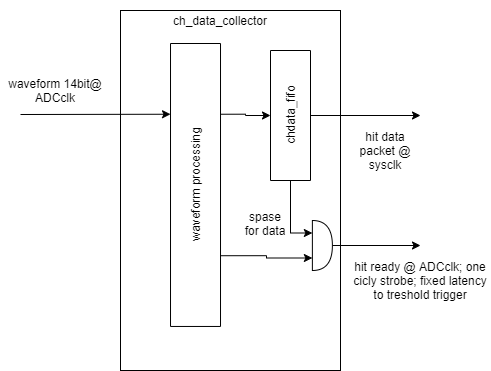
\includegraphics[width=0.5\textwidth]{ADC_event_collection.png}
	\caption{\label{fig:1} Data collecting scheme for single channel}
\end{figure}

\begin{table}[H]
\centering
\begin{tabular}{| l | l | l | l | l | l |}
\hline
word & 79 .. 72 & 71 .. 64 & 63 .. 34 & 33 .. 16 & 15 .. 0 \\ \hline
1 & waveform points number & channel & 0x0 & signal charge & waveform zero level \\ \hline
\end{tabular}
\caption{hit packet header.\label{tab2}}
\end{table}

\begin{table}[H]
\centering
\begin{tabular}{| l | l | l | l | l | l |}
\hline
word & 79 .. 64 & 63 .. 48 & 47 .. 32 & 31 .. 16 & 15 .. 0 \\ \hline
1 & 0x0 & waveform point n & waveform point n+1 & waveform point n+2 & waveform point n+3 \\ \hline
\end{tabular}
\caption{hit packet data word.\label{tab2}}
\end{table}


todo: wf points num to data words num

todo: fit procedure implementing in waveform processing

\subsection{Data collecting from channels fifo}

\begin{figure}[H]
	\centering 
	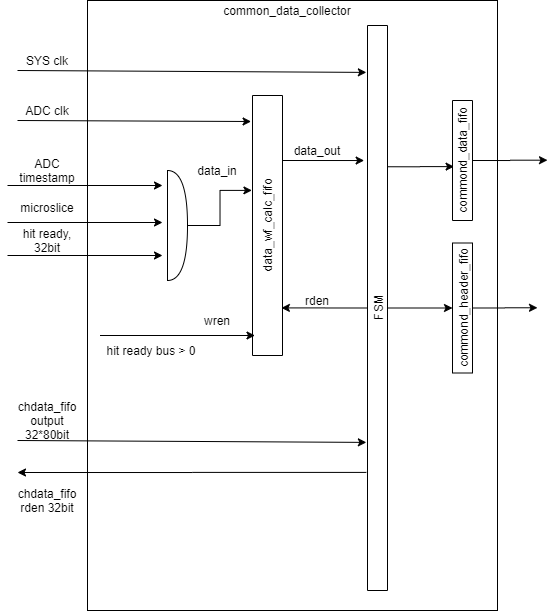
\includegraphics[width=0.5\textwidth]{ADC_common_event_collection.png}
	\caption{\label{fig:1} Data collecting scheme from all channels fifos}
\end{figure}




\end{document}

